\documentclass[border=10pt]{standalone}
\usepackage[utf8]{inputenc}
\usepackage[T1]{fontenc}
\usepackage{tikz}
\usepackage{xcolor}

\usetikzlibrary{arrows.meta, positioning, calc, fit}

\definecolor{globalq}{HTML}{E8E8E8}
\definecolor{localq}{HTML}{D4E8FF}
\definecolor{workercolor}{HTML}{2266AA}
\definecolor{successorcolor}{HTML}{888888}
\definecolor{taskcolor}{HTML}{C8E6C9}
\definecolor{batchcolor}{HTML}{FFF3E0}
\definecolor{localgreen}{HTML}{2E7D32}

\tikzset{
    queue/.style={draw, thick, rounded corners=3pt, minimum width=3cm, minimum height=0.6cm, fill=globalq, font=\small\bfseries},
    localqueue/.style={draw, thick, rounded corners=3pt, minimum width=2cm, minimum height=0.5cm, fill=localq, draw=workercolor, font=\small\bfseries},
    worker/.style={draw, thick, rounded corners=3pt, minimum width=1.2cm, minimum height=0.5cm, fill=localq, draw=workercolor, font=\small\bfseries},
    task/.style={draw, thick, rounded corners=2pt, minimum width=0.5cm, minimum height=0.35cm, fill=taskcolor, font=\tiny\bfseries},
    myarrow/.style={-{Stealth[length=5pt]}, thick},
    dasharrow/.style={-{Stealth[length=5pt]}, thick, dashed, color=successorcolor},
    localarrow/.style={-{Stealth[length=5pt]}, thick, dashed, color=localgreen},
    batchbox/.style={draw, thick, dashed, rounded corners=3pt, fill=batchcolor, fill opacity=0.3},
}

\begin{document}
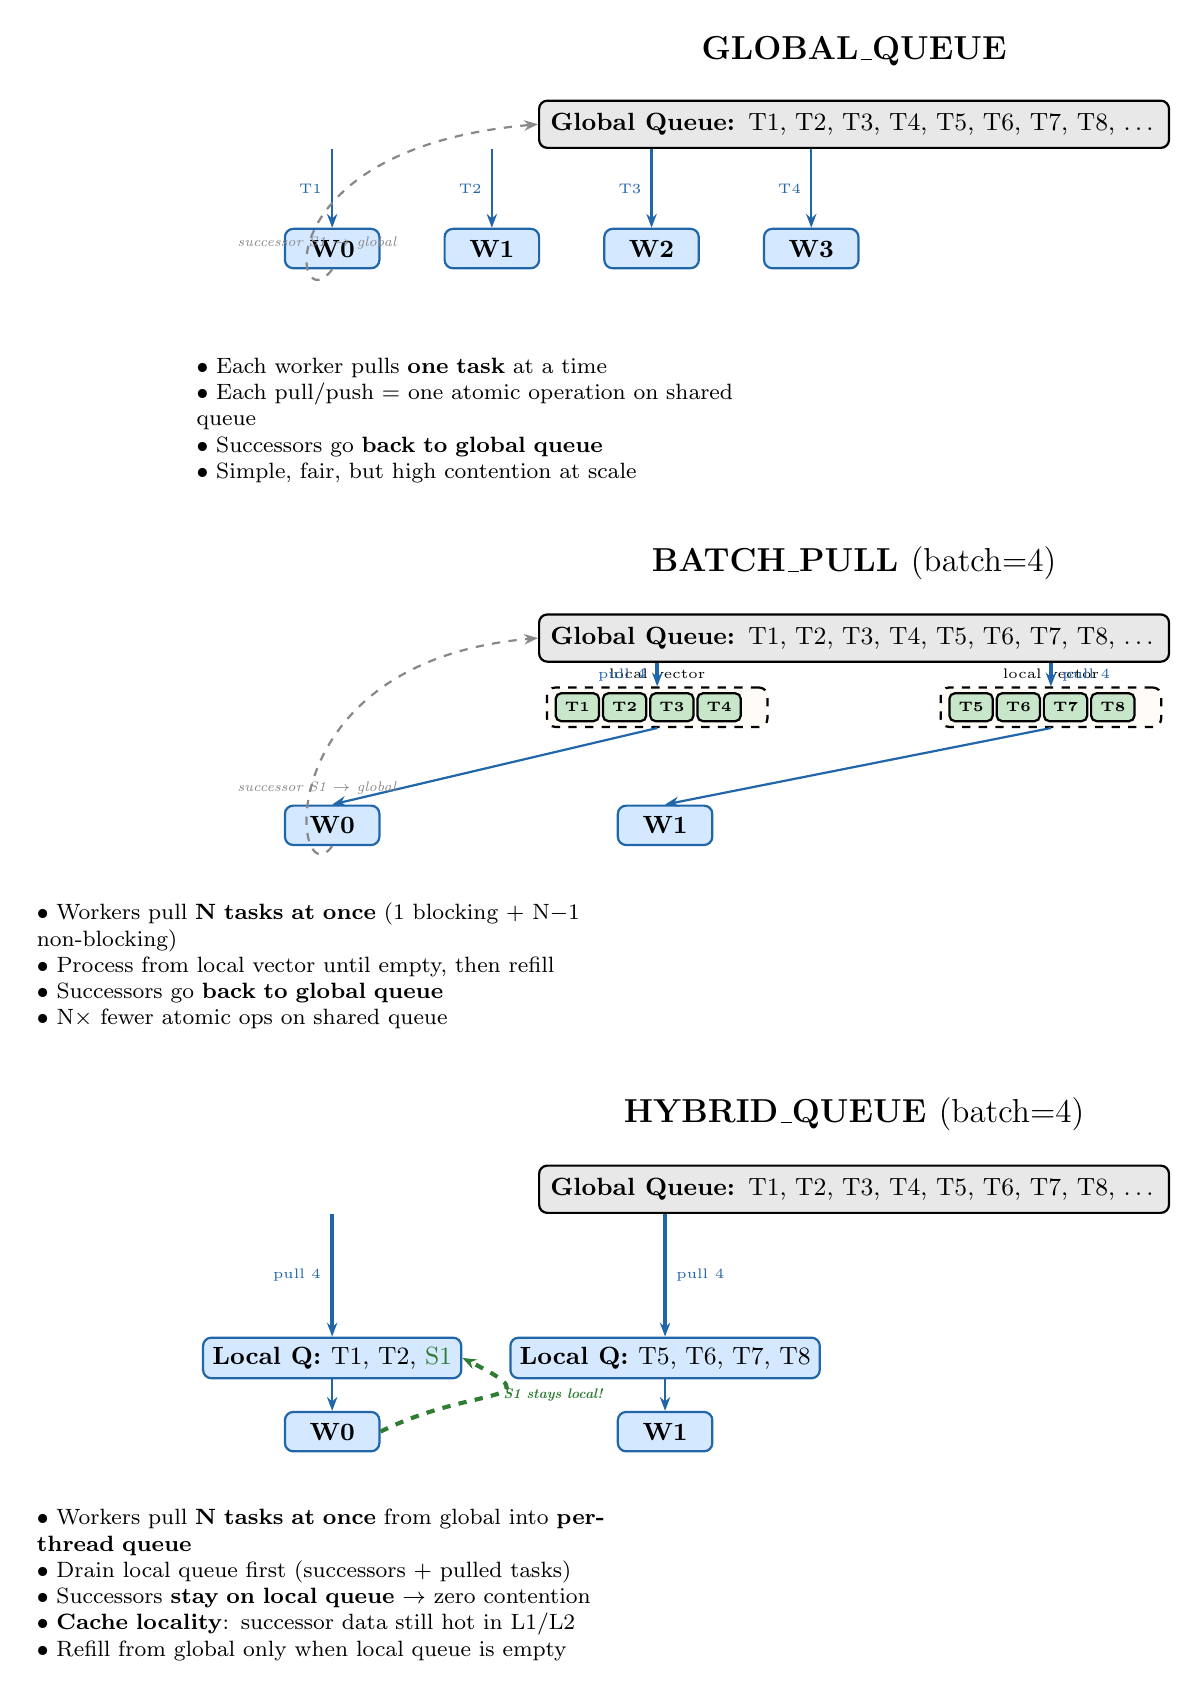
\begin{tikzpicture}[node distance=0.8cm and 1cm]

% ============================================================
% GLOBAL_QUEUE
% ============================================================
\node[font=\large\bfseries] (title1) at (0, 0) {GLOBAL\_QUEUE};

\node[queue, below=0.3cm of title1, minimum width=8cm] (gq) {Global Queue: \textnormal{T1, T2, T3, T4, T5, T6, T7, T8, \ldots}};

\node[worker, below left=1cm and 2cm of gq] (w0a) {W0};
\node[worker, right=0.8cm of w0a] (w1a) {W1};
\node[worker, right=0.8cm of w1a] (w2a) {W2};
\node[worker, right=0.8cm of w2a] (w3a) {W3};

\draw[myarrow, workercolor] (gq.south -| w0a) -- (w0a.north) node[midway, left, font=\tiny] {T1};
\draw[myarrow, workercolor] (gq.south -| w1a) -- (w1a.north) node[midway, left, font=\tiny] {T2};
\draw[myarrow, workercolor] (gq.south -| w2a) -- (w2a.north) node[midway, left, font=\tiny] {T3};
\draw[myarrow, workercolor] (gq.south -| w3a) -- (w3a.north) node[midway, left, font=\tiny] {T4};

\draw[dasharrow] (w0a.south) .. controls +(-0.5,-0.7) and +(-3.5,-0.3) .. (gq.west)
    node[pos=0.5, below, font=\tiny\itshape, text=successorcolor] {successor S1 $\rightarrow$ global};

\node[font=\footnotesize, text width=7.5cm, below=1cm of w1a, align=left] {
    $\bullet$ Each worker pulls \textbf{one task} at a time\\
    $\bullet$ Each pull/push = one atomic operation on shared queue\\
    $\bullet$ Successors go \textbf{back to global queue}\\
    $\bullet$ Simple, fair, but high contention at scale
};

% ============================================================
% BATCH_PULL
% ============================================================
\node[font=\large\bfseries] (title2) at (0, -6.5) {BATCH\_PULL \textnormal{(batch=4)}};

\node[queue, below=0.3cm of title2, minimum width=8cm] (gq2) {Global Queue: \textnormal{T1, T2, T3, T4, T5, T6, T7, T8, \ldots}};

\node[worker, below left=1.8cm and 2cm of gq2] (w0b) {W0};
\node[worker, right=3cm of w0b] (w1b) {W1};

% Batch boxes
\node[batchbox, below=0.3cm of gq2, xshift=-2.5cm, minimum width=2.8cm, minimum height=0.5cm] (batch0) {};
\node[font=\tiny, above=-0.02cm of batch0] {local vector};
\node[task] at ($(batch0.west)+(0.4,0)$) {T1};
\node[task] at ($(batch0.west)+(1.0,0)$) {T2};
\node[task] at ($(batch0.west)+(1.6,0)$) {T3};
\node[task] at ($(batch0.west)+(2.2,0)$) {T4};

\node[batchbox, below=0.3cm of gq2, xshift=2.5cm, minimum width=2.8cm, minimum height=0.5cm] (batch1) {};
\node[font=\tiny, above=-0.02cm of batch1] {local vector};
\node[task] at ($(batch1.west)+(0.4,0)$) {T5};
\node[task] at ($(batch1.west)+(1.0,0)$) {T6};
\node[task] at ($(batch1.west)+(1.6,0)$) {T7};
\node[task] at ($(batch1.west)+(2.2,0)$) {T8};

\draw[myarrow, workercolor, line width=1.5pt] (gq2.south -| batch0) -- (batch0.north) node[midway, left, font=\tiny] {pull 4};
\draw[myarrow, workercolor, line width=1.5pt] (gq2.south -| batch1) -- (batch1.north) node[midway, right, font=\tiny] {pull 4};

\draw[myarrow, workercolor] (batch0.south) -- (w0b.north);
\draw[myarrow, workercolor] (batch1.south) -- (w1b.north);

\draw[dasharrow] (w0b.south) .. controls +(-0.5,-0.7) and +(-3.5,-0.3) .. (gq2.west)
    node[pos=0.5, below, font=\tiny\itshape, text=successorcolor] {successor S1 $\rightarrow$ global};

\node[font=\footnotesize, text width=7.5cm, below=0.6cm of w0b, align=left] {
    $\bullet$ Workers pull \textbf{N tasks at once} (1 blocking + N$-$1 non-blocking)\\
    $\bullet$ Process from local vector until empty, then refill\\
    $\bullet$ Successors go \textbf{back to global queue}\\
    $\bullet$ N$\times$ fewer atomic ops on shared queue
};

% ============================================================
% HYBRID_QUEUE
% ============================================================
\node[font=\large\bfseries] (title3) at (0, -13.5) {HYBRID\_QUEUE \textnormal{(batch=4)}};

\node[queue, below=0.3cm of title3, minimum width=8cm] (gq3) {Global Queue: \textnormal{T1, T2, T3, T4, T5, T6, T7, T8, \ldots}};

\node[worker, below left=2.5cm and 2cm of gq3] (w0c) {W0};
\node[worker, right=3cm of w0c] (w1c) {W1};

% Per-thread queues
\node[localqueue, above=0.4cm of w0c, minimum width=3.2cm] (lq0) {Local Q: \textnormal{T1, T2, \textcolor{localgreen}{S1}}};
\node[localqueue, above=0.4cm of w1c, minimum width=3.2cm] (lq1) {Local Q: \textnormal{T5, T6, T7, T8}};

\draw[myarrow, workercolor, line width=1.5pt] (gq3.south -| lq0) -- (lq0.north) node[midway, left, font=\tiny] {pull 4};
\draw[myarrow, workercolor, line width=1.5pt] (gq3.south -| lq1) -- (lq1.north) node[midway, right, font=\tiny] {pull 4};

\draw[myarrow, workercolor] (lq0.south) -- (w0c.north);
\draw[myarrow, workercolor] (lq1.south) -- (w1c.north);

% Successor stays local
\draw[localarrow, line width=1.5pt] (w0c.east) .. controls +(1.2,0.6) and +(1.2,-0.6) .. (lq0.east)
    node[pos=0.5, right, font=\tiny\bfseries\itshape, text=localgreen] {S1 stays local!};

\node[font=\footnotesize, text width=7.5cm, below=0.6cm of w0c, align=left] {
    $\bullet$ Workers pull \textbf{N tasks at once} from global into \textbf{per-thread queue}\\
    $\bullet$ Drain local queue first (successors + pulled tasks)\\
    $\bullet$ Successors \textbf{stay on local queue} $\rightarrow$ zero contention\\
    $\bullet$ \textbf{Cache locality}: successor data still hot in L1/L2\\
    $\bullet$ Refill from global only when local queue is empty
};

\end{tikzpicture}
\end{document}
